\documentclass[format=acmsmall,review,timestamp,urlbreakonhyphens]{acmart}

%\documentclass[aps,pre,twocolumn,showpacs,preprintnumbers,amsmath,amssymb]{revtex4-1}
%\documentclass[preprint,showpacs,preprintnumbers,amsmath,amssymb]{revtex4}


\usepackage{graphicx}% Include figure files
\usepackage{dcolumn}% Align table columns on decimal point
\usepackage{bm}% bold math

\usepackage{xcolor}
\PassOptionsToPackage{dvipsnames}{xcolor}

\usepackage{amsfonts}
\usepackage{amsmath}
\usepackage{amssymb}
\usepackage{amsthm}
\usepackage{bbold}
\usepackage[american]{babel}
\usepackage[utf8]{inputenc}
\usepackage[OT1]{fontenc}
\usepackage{longtable}
%\usepackage[dvips]{graphicx}
\usepackage{xspace}
\usepackage{bbm}
\usepackage[all]{xy}
%\usepackage{slashbox}
%\usepackage[justification=centering]{caption}
\providecommand{\begeq}[1]{\begin{equation}#1\end{equation}}
\DeclareMathOperator{\tr}{tr}
\providecommand{\norm}[1]{\lVert#1\rVert}
\newtheorem{theorem}{Theorem}
\newtheorem{lemma}{Lemma}
\newtheorem{defi}{Definition}
\newtheorem{rem}{Remark}
\newtheorem{conj}{Conjecture}
\newtheorem{prop}{Proposition}
\DeclareMathOperator{\con}{cond}
\DeclareMathOperator{\diag}{diag}
\newcolumntype{C}[1]{>{\centering\arraybackslash}p{#1}}

% \newcommand{\michael}[1]{\textcolor{olive}{Michael: #1}}
% \newcommand{\christian}[1]{\textcolor{red}{Christian: #1}}

%Try to avoid widows and orphans
%\usepackage[all]{nowidow}
\clubpenalty = 10000
\widowpenalty = 10000
\displaywidowpenalty = 10000



\begin{document}

\acmJournal{TOMS}

% TODO update after acceptance
\acmVolume{0}
\acmNumber{0}
\acmArticle{0}
\acmYear{0000}
\acmMonth{0}

\citestyle{acmauthoryear}

% TODO
\keywords{}

% TODO
% CCScodes ....



% abstract must preced title in acmart style
\begin{abstract}
In scientific computing, the acceleration of atomistic computer simulations by means of custom hardware is finding ever growing application.
%Accelerating atomistic computer simulations using hardware acceleration is finding ever growing application in scientific computing.
A major limitation, however, is that the high efficiency in terms of performance and low power consumption entails the massive usage of low-precision computing units. Here, based on the approximate computing paradigm, we present an algorithmic method to rigorously compensate for numerical inaccuracies due to low-accuracy arithmetic operations, yet still obtaining exact expectation values using a properly modified Langevin-type equation. %By this, we lay the foundation for the development of efficient MD accelerators.
\end{abstract}



\title{Accurate Sampling with Noisy Forces from Approximate Computing}

\author{Varadarajan Rengaraj}
\affiliation{%
  \institution{Paderborn University}
  \department{Dynamics of Condensed Matter}
  \department{Department of Computer Science}
  \streetaddress{Warburger Str. 100}
  \city{Paderborn}
  \postcode{33098}
  \country{Germany}}
\email{rengaraj@campus.uni-paderborn.de}

\author{Michael Lass}
\orcid{0000-0002-5708-7632}
\affiliation{%
  \institution{Paderborn University}
  \department{Department of Computer Science}
  \department{Paderborn Center for Parallel Computing}
  \streetaddress{Warburger Str. 100}
  \city{Paderborn}
  \postcode{33098}
  \country{Germany}}
\email{michael.lass@uni-paderborn.de}

\author{Christian Plessl}
\orcid{0000-0001-5728-9982}
\affiliation{%
  \institution{Paderborn University}
  \department{Department of Computer Science}
  \department{Paderborn Center for Parallel Computing}
  \streetaddress{Warburger Str. 100}
  \city{Paderborn}
  \postcode{33098}
  \country{Germany}}
\email{christian.plessl@uni-paderborn.de}

\author{Thomas D. K\"uhne}
\orcid{0000-0001-5471-2407}
\affiliation{%
  \institution{Paderborn University}
  \department{Dynamics of Condensed Matter}
  \department{Center for Sustainable Systems Design}
  \department{Paderborn Center for Parallel Computing}
  \position{Chair of Theoretical Chemistry}
  \streetaddress{Warburger Str. 100}
  \city{Paderborn}
  \postcode{33098}
  \country{Germany}}
\email{tdkuehne@mail.upb.de}


%\date{\today}% It is always \today

             %\preprint{APS/123-QED}


%A Valid PACS numbers may be entered using the \verb+\pacs{#1}+ command.
%\pacs{31.15.-p, 31.15.Ew, 71.15.-m, 71.15.Pd}% PACS, the Physics and Astronomy
                             % Classification Scheme.
\maketitle


%%%%%%%%%%%%%%%%%%%%%%%%%%%%%%%%%%%%%%%%%%%%%%%%%%%%%%%%%%%%%%%%%%%%%%%%%%%%%%%%%%%%%%%%%%
\section{Introduction}
%%%%%%%%%%%%%%%%%%%%%%%%%%%%%%%%%%%%%%%%%%%%%%%%%%%%%%%%%%%%%%%%%%%%%%%%%%%%%%%%%%%%%%%%%%

Molecular dynamics (MD) is a very powerful and widely used technique to study thermodynamic equilibrium properties, as well as the real-time dynamics of complex systems made up of interacting atoms \cite{AlderWainwright1957}. This is done by numerically solving Newton's equations of motion in a time-discretized fashion via computing the nuclear forces of all atoms at every time step \cite{RahmanMD}. Computing these forces by analytically differentiating the interatomic potential with respect to the nuclear coordinates is computationally rather expensive, which is particularly true for electronic structure based \textit{ab-initio} MD simulations \cite{CPMD, CPMD_TDK, PayneRMP, WIRES_TDK}.

For a long time newly developed microchips became faster and more efficient over time due to new manufacturing processes and shrinking transistor sizes. However, this development slowly comes to an end as scaling down the structures of silicon based chips becomes more and more difficult. The focus therefore shifts towards making efficient use of the available technology. Hence, beside algorithmic developments \cite{MTS, Snir, GSE, Shaw, VerletCell, pSHAKE, John, Prodan}, there have been numerous custom computing efforts in this area to increase the efficiency of MD simulations by means of hardware acceleration, which we take up in this work. Examples of the latter are MD implementations on graphics processing units (GPUs) \cite{HOOMD, NAMD, OpenMM, HalMD, Lammps, Amber, Gromacs}, field-programmable gate arrays (FPGAs) \cite{HerbordtI, HerbordtII}, and application-specific integrated circuits (ASICs) \cite{AntonI, AntonII}.
%especially the ones based on graphics processing unit (GPU) and field-programmable gate array (FPGA).
While the use of GPUs for scientific applications is relatively widespread \cite{GPUcomp,Binder,Weigel}, the use of ASICs \cite{QCDScience, QCDOC, GrapeScience, Grape} and FPGAs is less common \cite{JanusI, JanusII, Convey, FDTD, Kenter, Galerkin}, but gained attention over the last years.
%Another approach is the use of accelerator hardware in the form of graphics processing units (GPUs), application-specific integrated circuits (ASICs) or field-programmable gate arrays (FPGAs). While the use of GPUs for scientific applications is relatively wide-spread, the use of ASICs and FPGAs is less common but gained attention over the last years.
In general, to maximize the computational power for a given silicon area, or equivalently minimize the power-consumption per arithmetic operation, more and more computing units are replaced with lower-precision units. This trend is mostly driven by market considerations of the gaming and artificial intelligence industries, which are the target customers of hardware accelerators and naturally do not absolutely rely on full computing accuracy.

%Microchips sizes of FPGA and GPU, are on a constant decline to accommodate more transistors but it also makes the transistors susceptible to both temporary and permanent failures. These hardware faults occasionally propagate to the software and considering this aspect, there is a renewed interest in approximate computing that can be applied in the software to give us the outputs that does not diverge too much from the ideal outputs. Approximate computing also ensures that the portion of investment needed in detecting the hardware faults, avoidance and recovery is avoided.

In the approach presented in this paper, we make effective use of low-precision special-purpose hardware for general-purpose scientific computing by leveraging the approximate computing (AC) paradigm~\cite{KlavikMalossiBekasEtAl2014, PlesslAC}. The general research goal of AC is to devise and explore ingenious techniques to relax the exactness of a calculation to facilitate the design of more powerful and/or more efficient computer systems. However, in scientific computing, where the exactness of all computed results is of paramount importance, attenuating accuracy requirements is not an option. Yet, we will demonstrate that it is nevertheless possible to rigorously compensate for numerical inaccuracies due to low-accuracy arithmetic operations and still obtain exact expectation values as obtained by ensemble averages of a properly modified Langevin equation.

%In this paper, we demonstrate the resilience of MD, simulating the use of low-precision data types. By this, we lay the foundation for the development of efficient MD accelerators.

The remainder of the paper is organized as follows. In Section~\ref{sec:ac} we revisit the basic principles of AC before introducing our modified Langevin equation in Section~\ref{sec:methodology}. Thereafter, in Section~\ref{sec:computational}, we describe the computational details of computational experiments. Our results are presented and discussed in Section~\ref{sec:results} before concluding the paper in Section~\ref{sec:conclusion}.

%In this paper, we describe one such technique that relaxes the exactness of the output and we explore to what extent it diverges from the ideal output.

%%%%%%%%%%%%%%%%%%%%%%%%%%%%%%%%%%%%%%%%%%%%%%%%%%%%%%%%%%%%%%%%%%%%%%%%%%%%%%%%%%%%%%%%%%
\section{Approximate Computing}
%%%%%%%%%%%%%%%%%%%%%%%%%%%%%%%%%%%%%%%%%%%%%%%%%%%%%%%%%%%%%%%%%%%%%%%%%%%%%%%%%%%%%%%%%%
\label{sec:ac}
%\subsection{Common number formats and their support in hardware}

A basic method of approximation and a key requirement for efficient use of processing hardware is the use of adequate data widths in computationally intensive kernels. While in many scientific applications the use of double-precision floating-point is most common, this precision is not always required.
%For example, iterative methods can exhibit resilience against low precision arithmetic~\cite{Strzodka2006, Bekas, Dongarra2017, lass17-esl, Dongarra2018, LassAC}.
For example, iterative methods can exhibit resilience against low precision arithmetic as has been shown for the computation of inverse matrix roots~\cite{lass17-esl} and for solving systems of linear equations~\cite{KlavikMalossiBekasEtAl2014,Bekas,Dongarra2017,Dongarra2018}.
Mainly driven by the growing popularity of artificial neural networks \cite{Gupta2015}, we can observe growing support of low-precision data types %, such as half-precision floating point and bfloat16,
in hardware accelerators.
%
In fact, recent GPUs targeting the data center have started supporting half-precision as well, nearly doubling the peak performance compared to single-precision and quadrupling it compared to double-precision arithmetics~\cite{tesla}. However, due to the low number of exponent bits, half-precision only provides a very limited dynamic range. In contrast, \texttt{bfloat16} provides the same dynamic range as single-precision, and just reduces precision. It is currently supported by Google's Tensor Processing Units (TPU)~\cite{tpu} and support is announced for future Intel Xeon processors~\cite{xeon} and Intel AgileX FPGAs. A list of commonly used data types, together with the corresponding number of bits used to represent the exponent and the mantissa (incl. the implicit bit), are shown in Table~\ref{tab:float}.
%In recent time we see increased use of floating-point variants different to single-precision and double-precision.
\begin{table}
  \caption{Common floating-point formats}
  \label{tab:float}
  \begin{tabular}{lrr}
    Type & exponent bits & mantissa bits \\
    \hline
    IEEE 754 Quadruple-precision & 15 & 113 \\
    IEEE 754 Double-precision & 11 & 53 \\
    IEEE 754 Single-precision & 8 & 24 \\
    IEEE 754 Half-precision & 5 & 11 \\
    Bfloat16 (truncated IEEE single-precision)& 8 & 8
  \end{tabular}
\end{table}

%Hardware support for these formats are typically available for single- and double-precision. Due to the spread of machine learning applications, some modern GPUs targeting the data center start supporting half-precision as well, nearly doubling the peak performance compared to single-precision and quadrupling it compared to double-precision arithmetics~\cite{tesla}. However, due to the low number of exponent bits, half-precision only provides a very limited dynamic range. In contrast, bfloat16 provides the same dynamic range as single-precision, and just reduces precision. It is currently supported by Google's Tensor Processing Units (TPU)~\cite{tpu} and support is announced for future Intel Xeon processors~\cite{xeon}.

Yet, programmable hardware such as FPGAs, as a platform for custom-built accelerator designs \cite{Strzodka2006, KenterVector, KenterPragma}, can make effective use of all of these, but also entirely custom number formats.
%The benefit of using low-precision types in terms of peak performance and resource utilization are not as foreseeable as on fixed hardware architectures, but instead depends on how efficiently the given hardware specification can be mapped to hardware elements on the FPGA. However, similar speedups as for CPUs and GPUs can often be achieved.
Developers can specify the number of exponent and mantissa bits and trade off precision against the amount of memory blocks required to store values and the number of logic elements required to perform arithmetic operations on them.

In addition to floating-point formats, also fixed-point representations can be used. Here, all numbers are stored as integers of fixed size with a
predefined scaling factor. Calculations are thereby performed using integer arithmetic. On CPUs and GPUs only certain models can perform integer operations with a peak performance similar to that of floating-point arithmetic, depending on the capabilities of the vector units / stream processors. Nevertheless, FPGAs typically can perform integer operations with performance similar to or even higher than that of floating-point. Due to the high flexibility of FPGAs with respect to different data formats and the possible use of entirely custom data types, we see them as the main target technology for our work. For this reason, we consider both floating-point and fixed-point arithmetic in the following.

%%%%%%%%%%%%%%%%%%%%%%%%%%%%%%%%%%%%%%%%%%%%%%%%%%%%%%%%%%%%%%%%%%%%%%%%%%%%%%%%%%%%%%%%%%
\section{Methodology}
%%%%%%%%%%%%%%%%%%%%%%%%%%%%%%%%%%%%%%%%%%%%%%%%%%%%%%%%%%%%%%%%%%%%%%%%%%%%%%%%%%%%%%%%%%
\label{sec:methodology}
To demonstrate the concept of approximate computing, we introduce white noise to the interatomic forces that are computed while running the MD simulation. In this section, we describe in detail on how we introduce the noise to mimic in software the behaviour that would happen when running the MD on the actual FPGA or GPU hardware with reduced numerical precision. We classify the computational errors into two types: fixed-point errors, and floating-point errors. Assuming that $\textbf{F}_{I}$ are the exact and $\textbf{F}_{I}^{N}$ the noisy forces from a MD simulations with low precision on a FPGA for instance, fixed-point errors can by modelled by

\begin{equation}
%\begin{pmatrix}
%\textbf{F}_{I}^{N(x)}\\
%\textbf{F}_{I}^{N(y)}\\
%\textbf{F}_{I}^{N(z)}\\
%\end{pmatrix} =
\textbf{F}_{I}^{N}=
\begin{pmatrix}
\text{F}_{I}^{x}\\
\text{F}_{I}^{y}\\
\text{F}_{I}^{z}\\
\end{pmatrix} +
\begin{pmatrix}
c_{1} \times 10^{-\beta }\\
c_{2} \times 10^{-\beta }\\
c_{3} \times 10^{-\beta }\\
\end{pmatrix}
,
\end{equation}
whereas floating-point errors are described by
\begin{equation}
%\begin{pmatrix}
%\textbf{F}_{I}^{N(x)}\\
%\textbf{F}_{I}^{N(y)}\\
%\textbf{F}_{I}^{N(z)}\\
%\end{pmatrix} =
\textbf{F}_{I}^{N} =
\begin{pmatrix}
\text{F}_{I}^{x} \times 10^{-\alpha_1}\\
\text{F}_{I}^{y} \times 10^{-\alpha_2}\\
\text{F}_{I}^{z} \times 10^{-\alpha_3}\\
\end{pmatrix} +
\begin{pmatrix}
c_{1} \times 10^{-(\alpha_1+\beta)}\\
c_{2} \times 10^{-(\alpha_2+\beta)}\\
c_{3} \times 10^{-(\alpha_3+\beta)}\\
\end{pmatrix}
.
\end{equation}
Therein, $c_1$, $c_2$ and $c_3$ are random values chosen in the range [-0.5, 0.5], whereas $\text{F}_{I}^{x}$, $\text{F}_{I}^{y}$ and $\text{F}_{I}^{x}$ are the individual force components of $\textbf{F}_{I}$, respectively. The floating-point scaling factor is denoted as $\alpha$ and the magnitude of the applied noise by \(\beta\).
%as discussed in detail in the computational details section. \(\textbf{F}_{I}\) is the exact consistent force and \(\textbf{F}_{I}^{FPGA}\) is the force computed when MD is run on the FPGA.

To rigorously correct the errors introduced by numerical noise we employ a modified Langevin equation. In particular, we model the force as obtained by a low-precision computation on a GPU or FPGA-based accelerator as
%we assume at this point a computational error \(\mathbf{\Xi }_{I}^{N}\) is added to the force that is computed and the force that we get at the output is not the exact force \(\textbf{F}_{I}\) but an approximation
\begin{equation} \label{fFPGA}
\textbf{F}_{I}^{N} = \textbf{F}_{I} + \mathbf{\Xi }_{I}^{N},
\end{equation}
where $\mathbf{\Xi }_{I}^{N}$ is an additive white noise for which
\begin{equation} \label{CrossCorr}
 \left \langle \textbf{F}_{I}\left ( 0 \right ) \mathbf{\Xi } _{I}^{N}\left ( t \right )\right \rangle \cong  0
\end{equation}
holds. Throughout, $\langle \cdots \rangle$ denotes Boltzmann-weighted ensemble averages as obtained by the partition function $Z=\text{Tr} \exp(-E/k_B T)$, where $E$ is the potential energy, $k_B$ the so-called Boltzmann constant, and $T$ the temperature. Given that $\mathbf{\Xi }_{I}^{N}$ is unbiased, which is in our case is true by its very definition, it is nevertheless possible to accurately sample the Boltzmann distribution by means of a Langevin-type equation \cite{Krajewski,Richters,Karhan}, which in its general form reads as
%Fortunately in our case, it is still possible to accurately obtain Boltzmann sampling by means of a modified Langevin equation
\begin{equation} \label{LangevinEq}
M_{I}\ddot{\textbf{R}}_{I}=\textbf{F}_{I}+\mathbf{\Xi }_{I}^{N}-\gamma _{N}M_{I}\dot{\textbf{R}}_{I},
\end{equation}
where $\dot{\textbf{R}}_{I}$ are the nuclear coordinates (the dot denotes time derivative), $M_I$ are the nuclear masses and $\gamma _{N}$ is a damping coefficient,
%where \(\textbf{R}_{I}\) are the positions of the atoms, \(M_{I}\) the corresponding atomic nuclear masses and \(\gamma _{N}\) is a friction coefficient
which is chosen to compensate for \(\mathbf{\Xi }_{I}^{N}\). The latter, in order to guarantee an accurate canonical sampling, has to obey
%\begin{equation}
% \left \langle \textbf{F}_{I}\left ( 0 \right ) \mathbf{\Xi } _{I}^{N}\left ( t \right )\right \rangle \cong  0,
%\end{equation}
the fluctuation-dissipation theorem
\begin{equation}
\left \langle \mathbf{\Xi }_{I}^{N}\left ( 0 \right ) \mathbf{\Xi }_{I}^{N}\left ( t \right ) \right \rangle \cong  2 \gamma_{N} M_I k_{B} T  \delta \left ( t \right ).
\label{FDT}
\end{equation}
%where $k_B$ is Boltzmann's constant, and $T$ is the desired temperature.

Substituting Eq.~\ref{fFPGA} into Eq.~\ref{LangevinEq} results in the desired modified Langevin equation
\begin{equation} \label{modLangevin}
M_{I}\ddot{\textbf{R}}_{I} = \textbf{F}_{I}^{N}-\gamma _{N}M_{I}\dot{\textbf{R}}_{I},
\end{equation}
which will be used throughout the remaining of this paper. This is to say that the noise, as originating from a low-precision computation, can be though of as the additive white noise of a thitherto unknown damping coefficient $\gamma_N$, which satisfies the fluctuation-dissipation theorem of Eq.~\ref{FDT}.  The specific value of $\gamma_N$ is determined in such a way so as to generate the correct average temperature, as measured by the equipartition theorem
\begin{equation}
\left\langle \frac{1}{2} M_I \dot{\textbf{R}}_{I} \right\rangle = \frac{3}{2} k_B T.
\label{EquiPartTheorem}
\end{equation}
%or in other words that the mean kinetic energy corresponds to the correct temperature $T$.

%We further present in this paper the method to effectively compensate for the additive noise introduced on the force using the existing langevin dynamics framework.



%%%%%%%%%%%%%%%%%%%%%%%%%%%%%%%%%%%%%%%%%%%%%%%%%%%%%%%%%%%%%%%%%%%%%%%%%%%%%%%%%%%%%%%%%%
\section{Computational details}
%%%%%%%%%%%%%%%%%%%%%%%%%%%%%%%%%%%%%%%%%%%%%%%%%%%%%%%%%%%%%%%%%%%%%%%%%%%%%%%%%%%%%%%%%%
\label{sec:computational}
To demonstrate our approach we have implemented it in the CP2K suite of programs \cite{cp2k}. More precisely, we have conducted MD simulations of liquid Silicon (Si) at 3000~K using the environment-dependent interatomic potential of Bazant et al. \cite{EIP1,EIP2}.
%The Empirical Interatomic Potential (EIP) calculation model for our MD simulation is Bazant potentials. The total number of Si atoms used for the MD simulation is thousand with a cubic cell length of 27.155 Angstrom.
All simulations consisted of 1000 Si atoms in a 3D-periodic cubic box of length 27.155~\AA. Using the algorithm of Ricci and Ciccotti \cite{Ricci}, Eq.~\ref{LangevinEq} was integrated with a discretized timestep of 1.0~fs with $\gamma_N = 0.001~$fs$^{-1}$.
%Langevin dynamics configured for the above settings have been run with frictional coefficient \(\gamma\) assigned a value equal to 1/1000 \(fs^{-1}\). This simulation run is considered as the reference with which the computational error introduced simulations are compared. As described in the Methodology section, computational errors are classified as fixed point error and floating point error. With necessary changes incorporated to the cp2k software, two different builds for the two variants of errors have been made and Langevin dynamics were performed on those builds.

Whereas the latter settings were used to compute our reference data, in total six different cases of fixed-point and floating-point errors were investigated by varying the exponent $\beta$ between 0 (huge noise) and 3 (tiny noise) that is, ranging from $1/1000$ of the physical force up to the same magnitude as the force. %tested and for the equation representing fixed point error, the corresponding \(\beta\) value that was used were 1, 2 and 3. Similarly three different cases of floating point errors were tested and for the equation representing floating point error, the corresponding \(\beta\) value that was used were 0, 1, 2.
As already alluded to above, the additive white noise is compensated by means of Eq.~\ref{modLangevin} by varying $\gamma_N$ on-the-fly using a Berendsen-like algorithm until the the equipartition theorem of Eq.~\ref{EquiPartTheorem} is satisfied \cite{Berendsen,TDKwater,TDKrev}. Alternatively, $\gamma_N$ can be computed by integrating the autocorrelation function of the additive white noise \cite{RZK}.
%As discussed earlier in the methodology section, a separate frictional coefficient is necessary to compensate for the computational error that was  introduced in the builds. This frictional coefficient is managed through the parameter called shadow \(\gamma\) and this parameter is available in the langevin section of the cp2k software.
In Table~\ref{tab:gamma} the resulting values of \textit{\(\gamma_N^{fix}\)} for fixed-point and \textit{\(\gamma_N^{float}\)} for floating-point errors are reported as a function of \textit{\(\beta\)}. %Units for \(\gamma\) and shadow \(\gamma\) is \(fs^{-1}\).
%\begin{table}[h!]
%\caption{Shadow \(\gamma\) values for the fixed point errors.}
%\begin{tabular}{|l|l|l|}
%\hline
%\textit{\(\beta\)} & \textit{\(\gamma_N^{fix}\)} & \textit{\(\gamma_N^{float}\)} \\ \hline
%0 & & 0.00025 \\ \hline
%1             & 0.0004  & 0.000005              \\ \hline
%2             & 0.000009    & 0.000005          \\ \hline
%3             & 0.0000009 &            \\ \hline
%\end{tabular}
%\end{table}
\begin{table}
  \caption{Values for \textit{\(\gamma_N^{fix}\)} and \textit{\(\gamma_N^{float}\)} as a function of \textit{\(\beta\)}.}
  \label{tab:gamma}
  \begin{tabular}{lrr}
    \textit{\(\beta\)} & \textit{\(\gamma_N^{fix}\)} & \textit{\(\gamma_N^{float}\)} \\
    \hline
    0 &           & 0.00025  \\
    1 & 0.0004    & 0.000005 \\
    2 & 0.000009  & 0.000005 \\
    3 & 0.0000009 &
  \end{tabular}
\end{table}

%\begin{table}[h!]
%\caption{Shadow \(\gamma\) values for the fixed point errors.}
%\begin{tabular}{|l|l|}
%\hline
%\textit{\(\beta\) } & \textit{\(\gamma_N^{}\)} \\ \hline
%1             & 0.0004                \\ \hline
%2             & 0.000009              \\ \hline
%3             & 0.0000009             \\ \hline
%\end{tabular}
%\end{table}

%\begin{table}[h!]
%\caption{Shadow \(\gamma\) values for the floating point errors.}
%\begin{tabular}{|l|l|}
%\hline
%\textit{\(\beta\) } & \textit{\(\gamma_N\)} \\ \hline
%0             & 0.00025               \\ \hline
%1             & 0.000005              \\ \hline
%2             & 0.000005              \\ \hline
%\end{tabular}
%\end{table}


%%%%%%%%%%%%%%%%%%%%%%%%%%%%%%%%%%%%%%%%%%%%%%%%%%%%%%%%%%%%%%%%%%%%%%%%%%%%%%%%%%%%%%%%%%
\section{Results and Discussion}
%%%%%%%%%%%%%%%%%%%%%%%%%%%%%%%%%%%%%%%%%%%%%%%%%%%%%%%%%%%%%%%%%%%%%%%%%%%%%%%%%%%%%%%%%%
\label{sec:results}
As can be directly deduced from Table~\ref{tab:gamma}, the smaller values of $\gamma_N$ for a given $\beta$ immediately suggest the higher noise resilience when using floating-point as compared to fixed-point numbers.
\begin{figure}%[h!]
\begin{center}
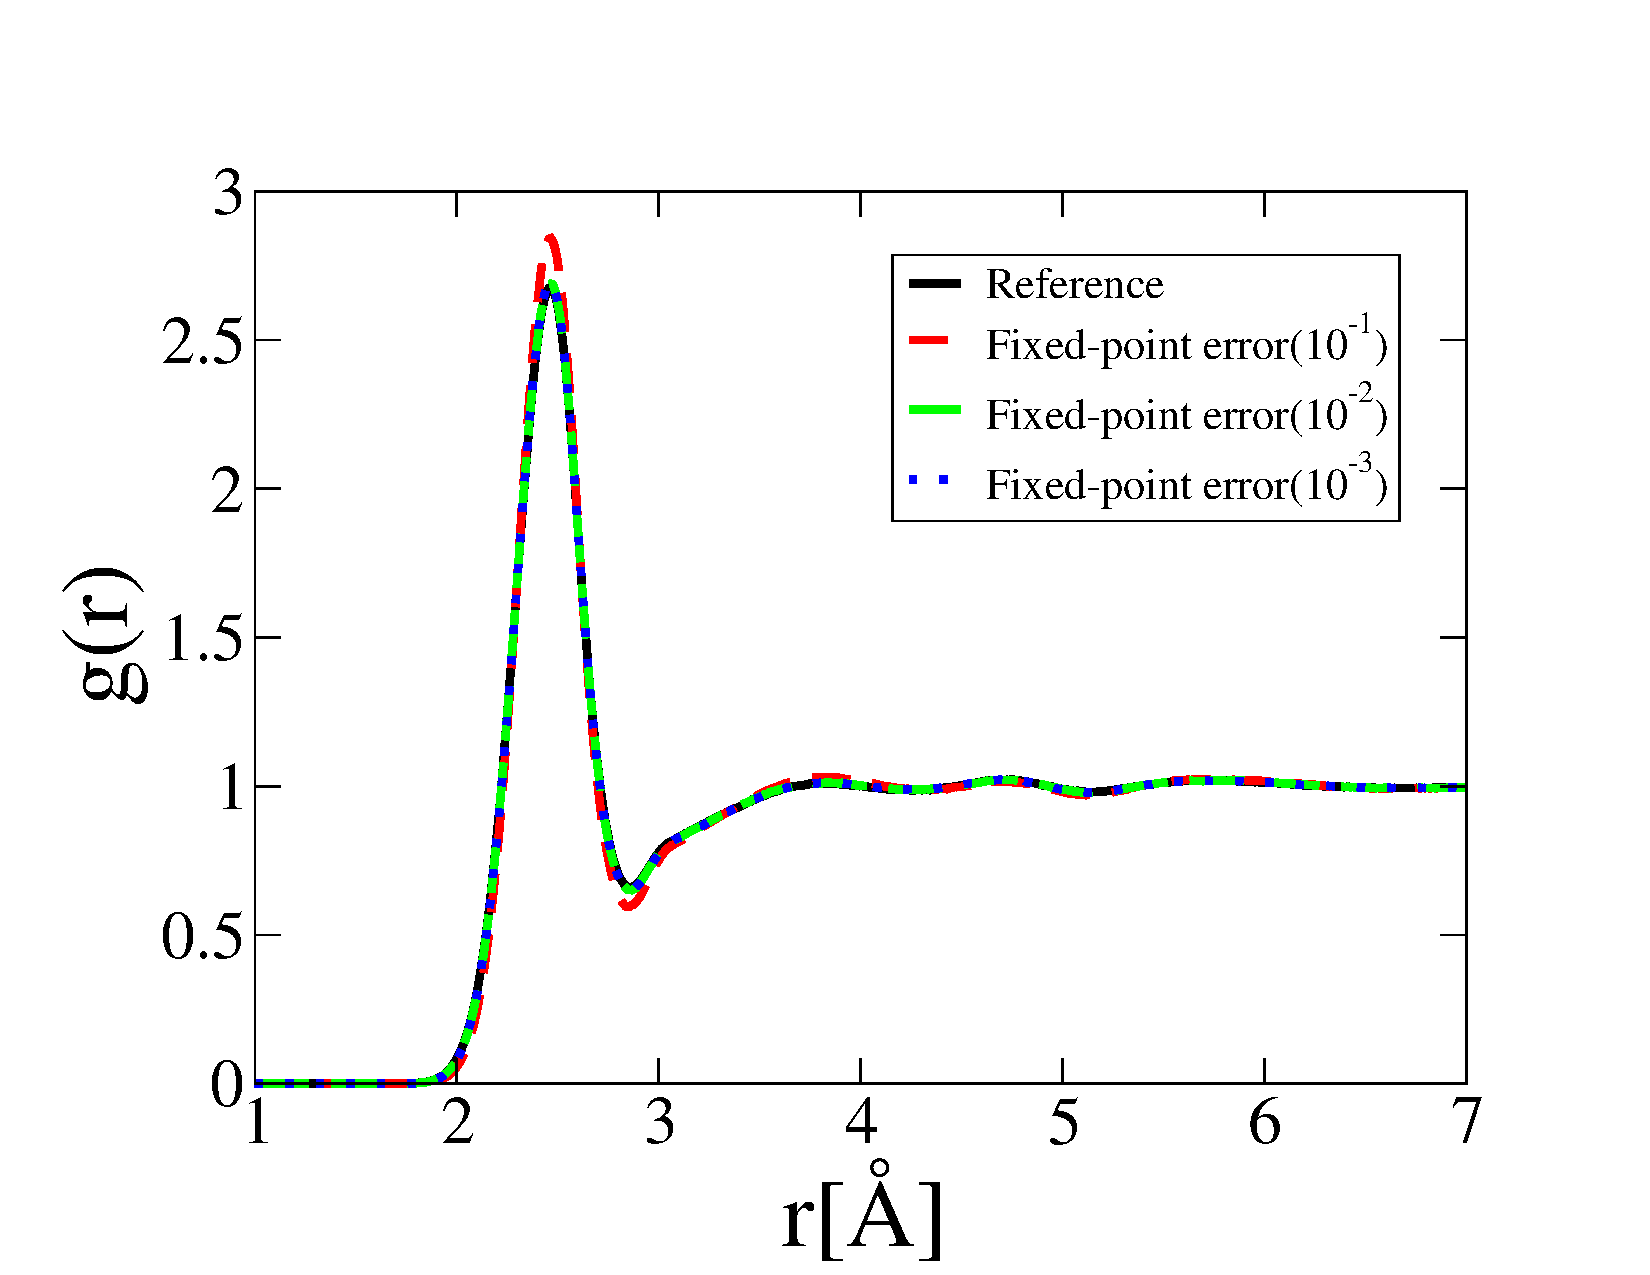
\includegraphics[width=0.475\textwidth]
{figures/Fixed_point_rdf2.pdf}
\end{center}
\caption{\label{Fig1}
Partial pair correlation function for liquid Si at 3000~K with noisy forces introduced by fixed-point errors of magnitude $10^{-3}$ (blue), $10^{-2}$ (green) and $10^{-1}$ (red). For comparison, the results, as obtained by our reference calculations without noise, are shown in black.
} \end{figure}
In Figs.~\ref{Fig1} and \ref{Fig2}, the Si-Si partial pair-correlation function $g(r)$, which describes how the particle-density varies as a function of distance from a reference particle (atoms, molecules, colloids, etc.), as computed using an optimal scheme for orthorombic systems \cite{KAF}, is shown for different values of $\beta$. %In Fig. 1 we show the pair correlation functions g(r) calculated with noisy forces generated from fixed-point errors. In Fig. 2 we show the pair correlation functions g(r) calculated with noisy forces generated with floating-point errors.
As can be seen, for both fixed-point and floating-point errors, the agreement with our reference calculation is nearly perfect up to the highest noise we have investigated. As already anticipated earlier, the usage of floating-point errors is not only able to tolerate higher noise levels, but is also throughout more accurate.
\begin{figure}%[h!]
\begin{center}
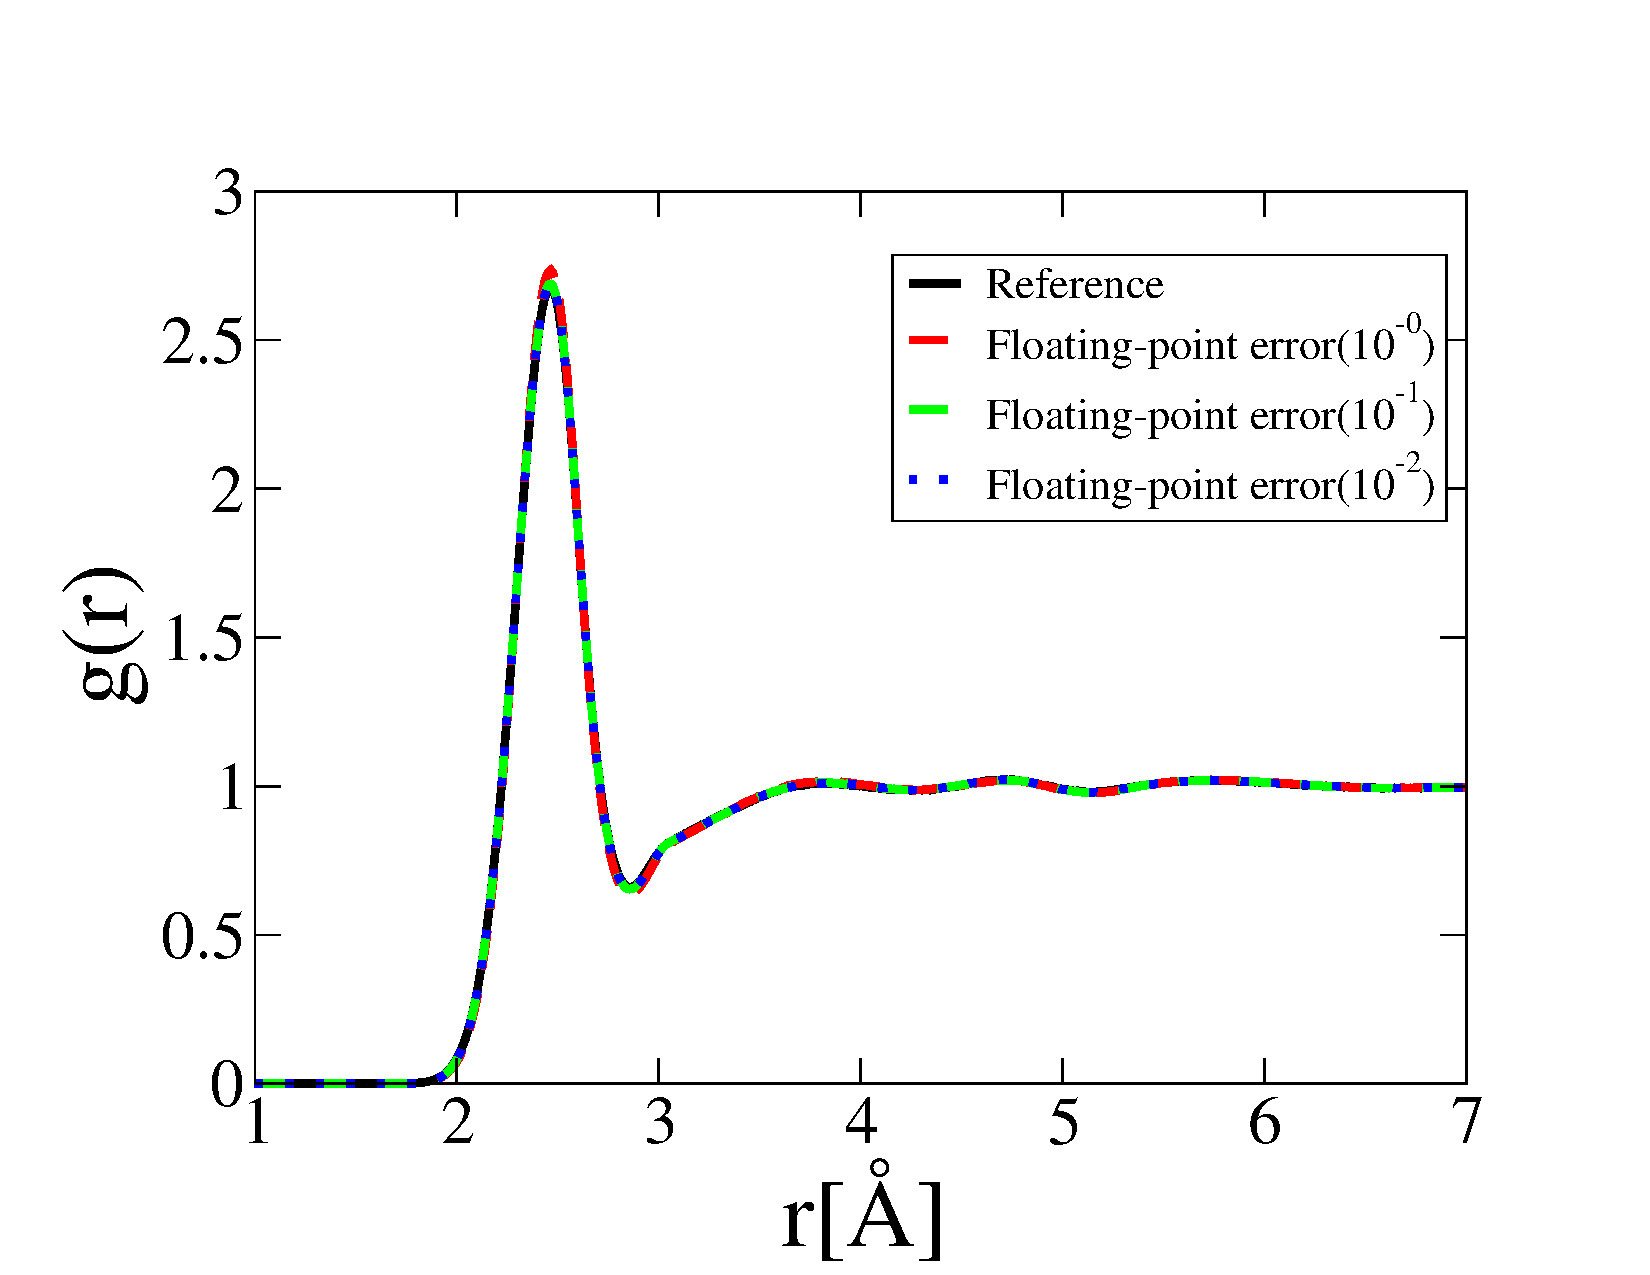
\includegraphics[width=0.475\textwidth]
{figures/Floating_point_rdf2.pdf}
\end{center}
\caption{\label{Fig2}
Partial pair correlation function for liquid Si at 3000~K with noisy forces introduced by floating-point errors of magnitude $10^{-2}$ (blue), $10^{-1}$ (green) and $10^{-0}$ (red). For comparison, the results, as obtained by our reference calculations without noise, are shown in black.
} \end{figure}

To verify that the sampling is indeed canonical, in Fig.~\ref{Fig3} the actual kinetic energy distribution as obtained by our simulations using noisy forces and compared to the analytic Maxwell distribution. It is evident that if sampled long enough, not only the mean value, but also the the distribution tails are in excellent agreement with the exact Maxwellian kinetic energy distribution, which demonstrates that we are indeed performing a canonical sampling.
\begin{figure}%[h!]
\begin{center}
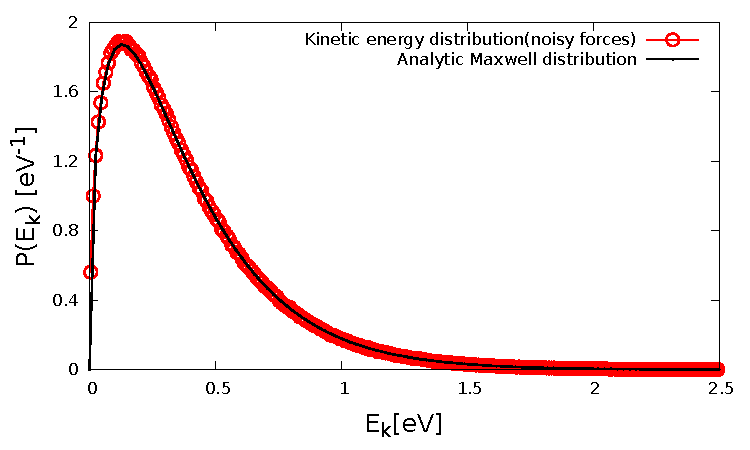
\includegraphics[width=0.475\textwidth]
{figures/maxwelldistribution_new.pdf}
\end{center}
\caption{\label{Fig3}
Kinetic energy distribution of liquid Si at 3000~K, as obtained by our simulations using noisy forces (circles). For comparison the analytic Maxwell distribution is also shown (line).
} \end{figure}
To further assess the accuracy of the present method, we expand the autocorrelation of the noisy forces, i.e.
%\begin{equation}
%\begin{split}
%\left \langle \textbf{F}_{I}^{N}\left ( 0 \right )\textbf{F}_{I}^{N}\left ( t \right )\right \rangle = \linebreak \\ \left \langle \left ( \textbf{F}_{I}\left ( 0 \right ) + \mathbf{\Xi } _{I}^{N}\left(0 \right )\right) \left( \textbf{F}_{I}\left ( t \right )+\mathbf{\Xi } _{I}^{N}\left ( t \right )\right) \right \rangle
%\end{split}
%\end{equation}
\begin{subequations}
\begin{eqnarray}
  && \left \langle \textbf{F}_{I}^{N}\left ( 0 \right )\textbf{F}_{I}^{N}\left ( t \right )\right \rangle \\
  &=& \left \langle \left ( \textbf{F}_{I}\left ( 0 \right ) + \mathbf{\Xi } _{I}^{N} \left(0 \right )\right) \left( \textbf{F}_{I}\left ( t \right )+\mathbf{\Xi } _{I}^{N}\left ( t \right )\right) \right \rangle \\
  &=& \left \langle \textbf{F}_{I}\left ( 0 \right ) \textbf{F}_{I}\left ( t \right )\right \rangle + \left \langle \textbf{F}_{I}\left ( 0 \right ) \mathbf{\Xi } _{I}^{N}\left(t \right )\right \rangle \label{AutoCorr} \\
  &+& \left \langle \textbf{F}_{I}\left ( t \right ) \mathbf{\Xi } _{I}^{N}\left(0 \right )\right \rangle + \left \langle \mathbf{\Xi } _{I}^{N}\left(0 \right ) \mathbf{\Xi } _{I}^{N}\left(t \right )\right \rangle.  \nonumber
\end{eqnarray}
\end{subequations}
%\begin{equation}\label{eq:1}
%\begin{split}
%\left \langle \textbf{F}_{I}^{N}\left ( 0 \right )\textbf{F}_{I}^{N}\left ( t \right )\right \rangle = \left \langle \textbf{F}_{I}\left ( 0 \right ) \textbf{F}_{I}\left ( t \right )\right \rangle + \linebreak \\\left \langle \textbf{F}_{I}\left ( 0 \right ) \mathbf{\Xi } _{I}^{N}\left(t \right )\right \rangle +  \left \langle \textbf{F}_{I}\left ( t \right ) \mathbf{\Xi } _{I}^{N}\left(0 \right )\right \rangle + \left \langle \mathbf{\Xi } _{I}^{N}\left(0 \right ) \mathbf{\Xi } _{I}^{N}\left(t \right )\right \rangle
%\end{split}
%\end{equation}
Since the cross correlation terms between the exact force and the additive white noise is vanishing due to Eq.~\ref{CrossCorr}, comparing the autocorrelation of the noisy forces $\langle \textbf{F}_{I}^{N}(0)\textbf{F}_{I}^{N}(t)\rangle$ with the autocorrelation of the exact forces $\langle \textbf{F}_{I}(0) \textbf{F}_{I}(t)\rangle$ permits to assess the localization of the last term of Eq.~\ref{AutoCorr}.
%Since, due to fluctuation-dissipation theorem, the last term of Eq.~\ref{AutoCorr} corresponds to a $\delta$-function, comparing the autocorrelation of the noisy forces $\langle \textbf{F}_{I}^{N}(0)\textbf{F}_{I}^{N}(t)\rangle$ with the autocorrelation of the exact forces $\langle \textbf{F}_{I}(0) \textbf{F}_{I}(t)\rangle$ permits to assess the cross correlation terms between the exact force and the additive white noise.
The fact that $\langle \textbf{F}_{I}^{N}(0)\textbf{F}_{I}^{N}(t)\rangle$ is essentially identical to $\langle \textbf{F}_{I}(0) \textbf{F}_{I}(t)\rangle$, as can be seen in Fig.~\ref{Fig4}, implies that $\langle \mathbf{\Xi } _{I}^{N}(0) \mathbf{\Xi } _{I}^{N}(t)\rangle$ is very close to a $\delta$-function as required by the fluctuation-dissipation theorem in order to ensure an accurate canonical sampling of the Boltzmann distribution. In other words, from this it follows that our initial assumption underlying Eq.~\ref{modLangevin}, to model the noise due to a low-precision calculation as an additive white noise channel, is justified.
\begin{figure}%[h!]
\begin{center}
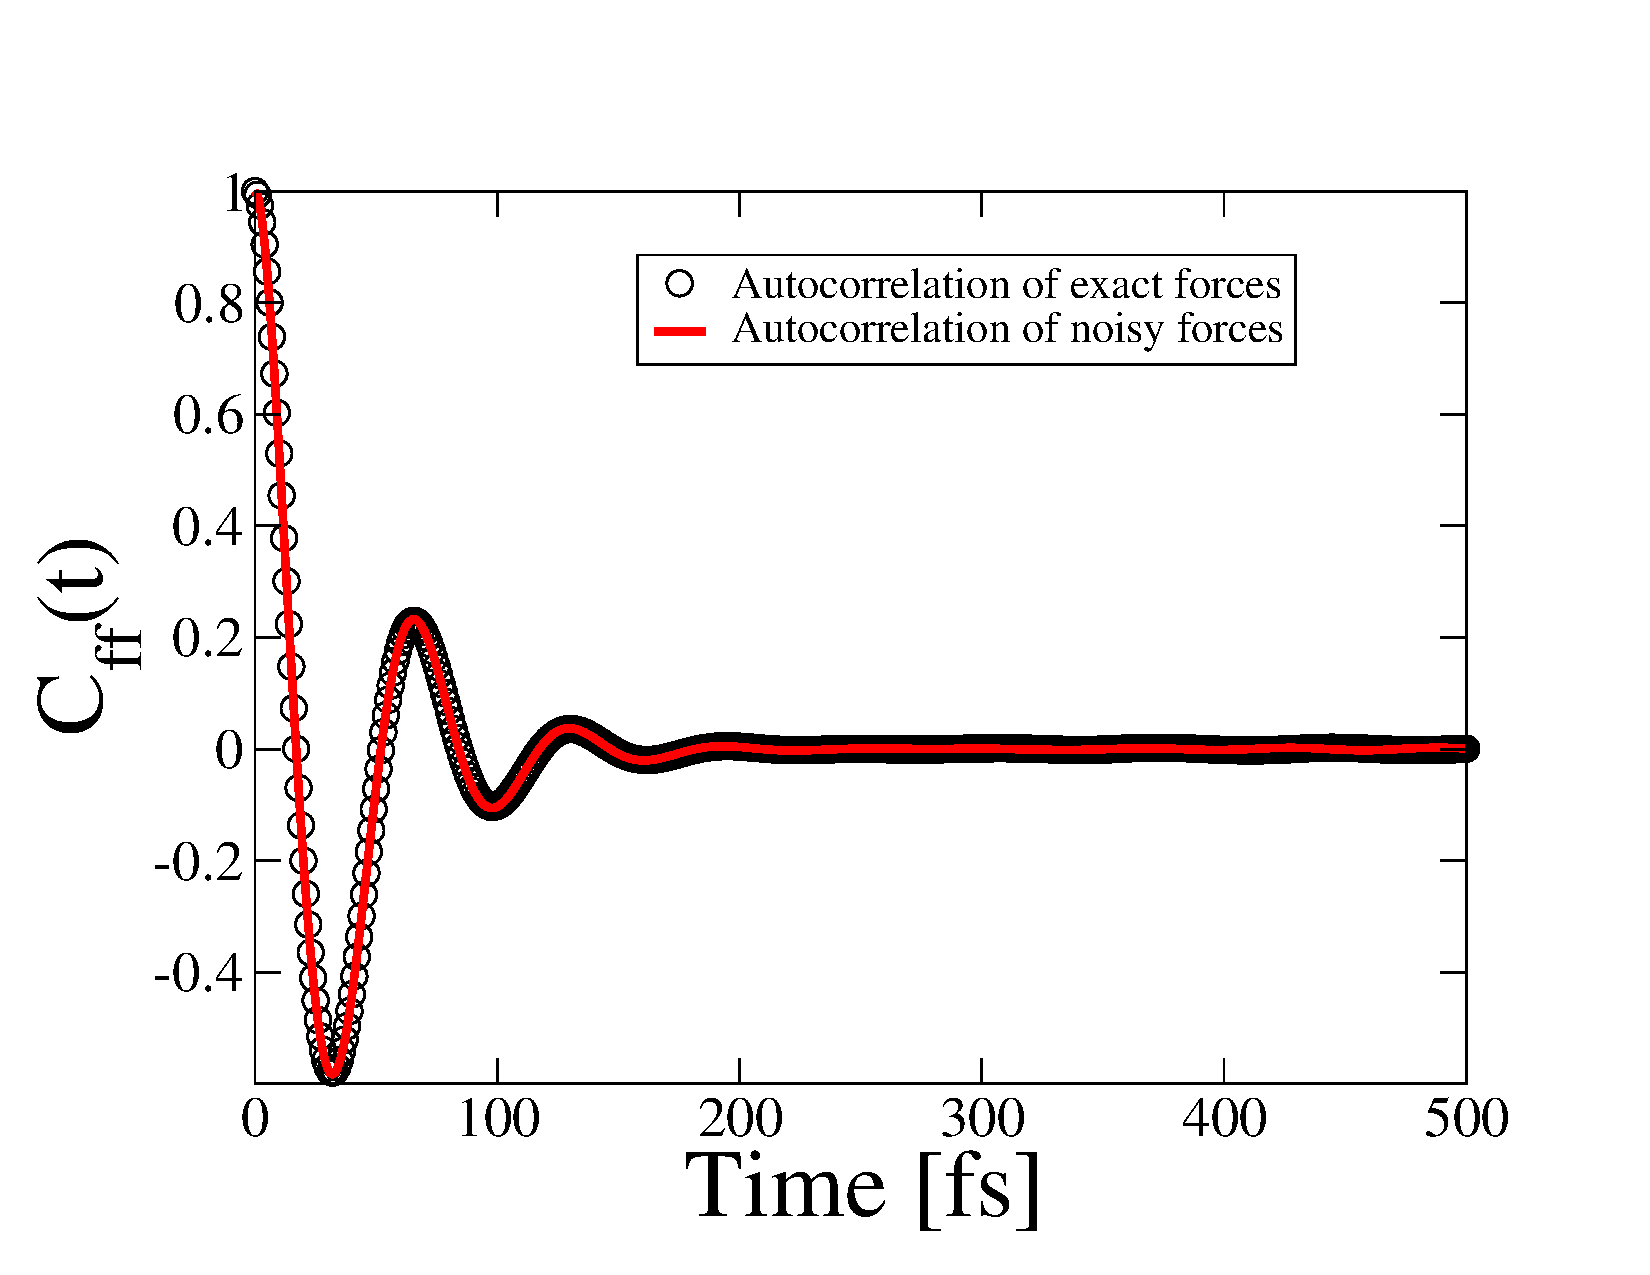
\includegraphics[width=0.475\textwidth]
{figures/AutocorrelationPlot_n.pdf}
\end{center}
\caption{\label{Fig4}
The Autocorrelation of the noisy forces \(
\left \langle \textbf{F}_{I}^{N}\left ( 0 \right ) \textbf{F}_{I}^{N}\left ( t \right )\right \rangle \)(line), which are compared to the autocorrelation of the exact forces \( \left \langle \textbf{F}_{I}\left ( 0 \right ) \textbf{F}_{I}\left ( t \right )\right \rangle \)(circles).
} \end{figure}

%If the random value that was used to generate the computational error is chosen in the range [0,1] instead of [-0.5,0.5], we encounter a phenomenon called "Flying Ice Cube" \cite{flyingIceCube} during our MD simulations.

%%%%%%%%%%%%%%%%%%%%%%%%%%%%%%%%%%%%%%%%%%%%%%%%%%%%%%%%%%%%%%%%%%%%%%%%%%%%%%%%%%%%%%%%%%
\section{Conclusion}
%%%%%%%%%%%%%%%%%%%%%%%%%%%%%%%%%%%%%%%%%%%%%%%%%%%%%%%%%%%%%%%%%%%%%%%%%%%%%%%%%%%%%%%%%%
\label{sec:conclusion}
%To summarize, in this paper, we described the method to compensate for the computational errors that are introduced when running the MD code in FPGA or GPU using approximate computing technique.
We conclude by noting that the present method have been recently implemented in the universal force engine i-Pi \cite{iPi}, which can be generally applied to all sorts of forces affected by stochastic noise such as those computed by GPUs or other hardware accelerators~\cite{HOOMD, NAMD, OpenMM, HalMD, Lammps, Amber, Gromacs}, and potentially even quantum computing devices \cite{Steane, Knill, Blatt, Chow}. The possibility to apply similar ideas to N-body simulations~\cite{White, Makino} and to combine it with further algorithmic approximations~\cite{LassAC} is to be underlined and will be presented elsewhere.



% TODO write grant sponsors.. with special environment, see acmart.pdf page 23
%\begin{acks}
%  The authors would like to thank Dr. Yuhua Li for providing the
%  matlab code of the \textit{BEPS} method.
%  The authors would also like to thank the anonymous referees for
%  their valuable comments and helpful suggestions. This work is
%  supported by the \grantsponsor{GS501100001809}{National Natural
%  Science Foundation of
%  China}{https://doi.org/10.13039/501100001809} under Grant
%  No.: ̃\grantnum{GS501100001809}{61273304}
%  and ̃\grantnum[http://www.nnsf.cn/youngscientists]{GS501100001809}{Young
%  Scientists’ Support Program}.
%\end{acks}

\begin{acks}
The authors would like to thank the Paderborn Center for Parallel Computing (PC2) for computing time on OCuLUS and FPGA-based supercomputer NOCTUA. Funding from the Paderborn University's research award for ``Green IT'' is kindly acknowledged. This project has received funding from the European Research Council (ERC) under the European Union's Horizon 2020 research and innovation programme (grant agreement No 716142).
\end{acks}

% The next two lines define the bibliography style to be used, and the bibliography file.
\bibliographystyle{ACM-Reference-Format}
\bibliography{report}

\end{document}
